
\subsection{Graphical Interface Interaction}

A graphical web interface was chosen as option of \TVB face for quick interaction. The web interface is easy to access (local or remotely),
it can be used by different types of users, including the ones without programming knowledge, and it offers great 
support while learning about \TVB concepts and workflow expectations. 
In our modeling diagrams, we called the actor accessing \TVB through the web interface a \emph{G-User}.

The http is served using \emph{Cherrypy} \texttt{http://www.cherrypy.org/} which is a minimalist, object-oriented web framework, 
in combination with \emph{Genshi} templating system, to support the separation of layers as guided by \emph{MVC (Model View Controller)} pattern.

	\subsubsection{Projects, Accounts, Operations \& Data}

\TVB uses entities like: Account, Project, Operation, DataType and Workflow, for modeling G-User actions and artifacts. 

 An \emph{Account} or \emph{User} is needed for accessing  \TVB through the web interface. 
 When \TVB web interface is fired for the first time, the G-User is requested to set the username and password for the first account.
Later on, people can \emph{register} for other accounts, but for using these new accounts they will need first to get validated by the 
initial account (which acts under \emph{admin} role).

A \emph{Project} in \TVB is a logical grouping entity, which  can be used in several ways by the end-user; 
for example one could choose to create a project for each experiment in \TVB, while others might create projects for each subject they simulate.
Each project has a single User (or Account) as owner, but a project can be shared with multiple other users.

Any execution of an Adapter results into an \emph{Operation} in the context of a project. Multiple operations will be executed under the same project.
For example we will have operations created for each execution of a simulation, each run of a Fourier analyzer, or launch of a Brain Visualizer.
An operation changes status over time, from \emph{started} into \emph{canceled}, \emph{finished successfully} or \emph{finished with error}.
One operation can have multiple input and output parameters and parameters can be scalars or DataTypes.

A \emph{Workflow} in \TVB is a set of operations with they artifacts, and wraps around a simulation as leading component.
A workflow can be seen as a default \emph{tag} placed by the system on operations and DataTypes 
which are logically connected, as resulting one after the other.
Custom tags can also be added by the end-user both on DataTypes and operations, for tracking data inside a TVB Project.
	
 \begin{figure*}
 	\centering
	\subfloat[][]{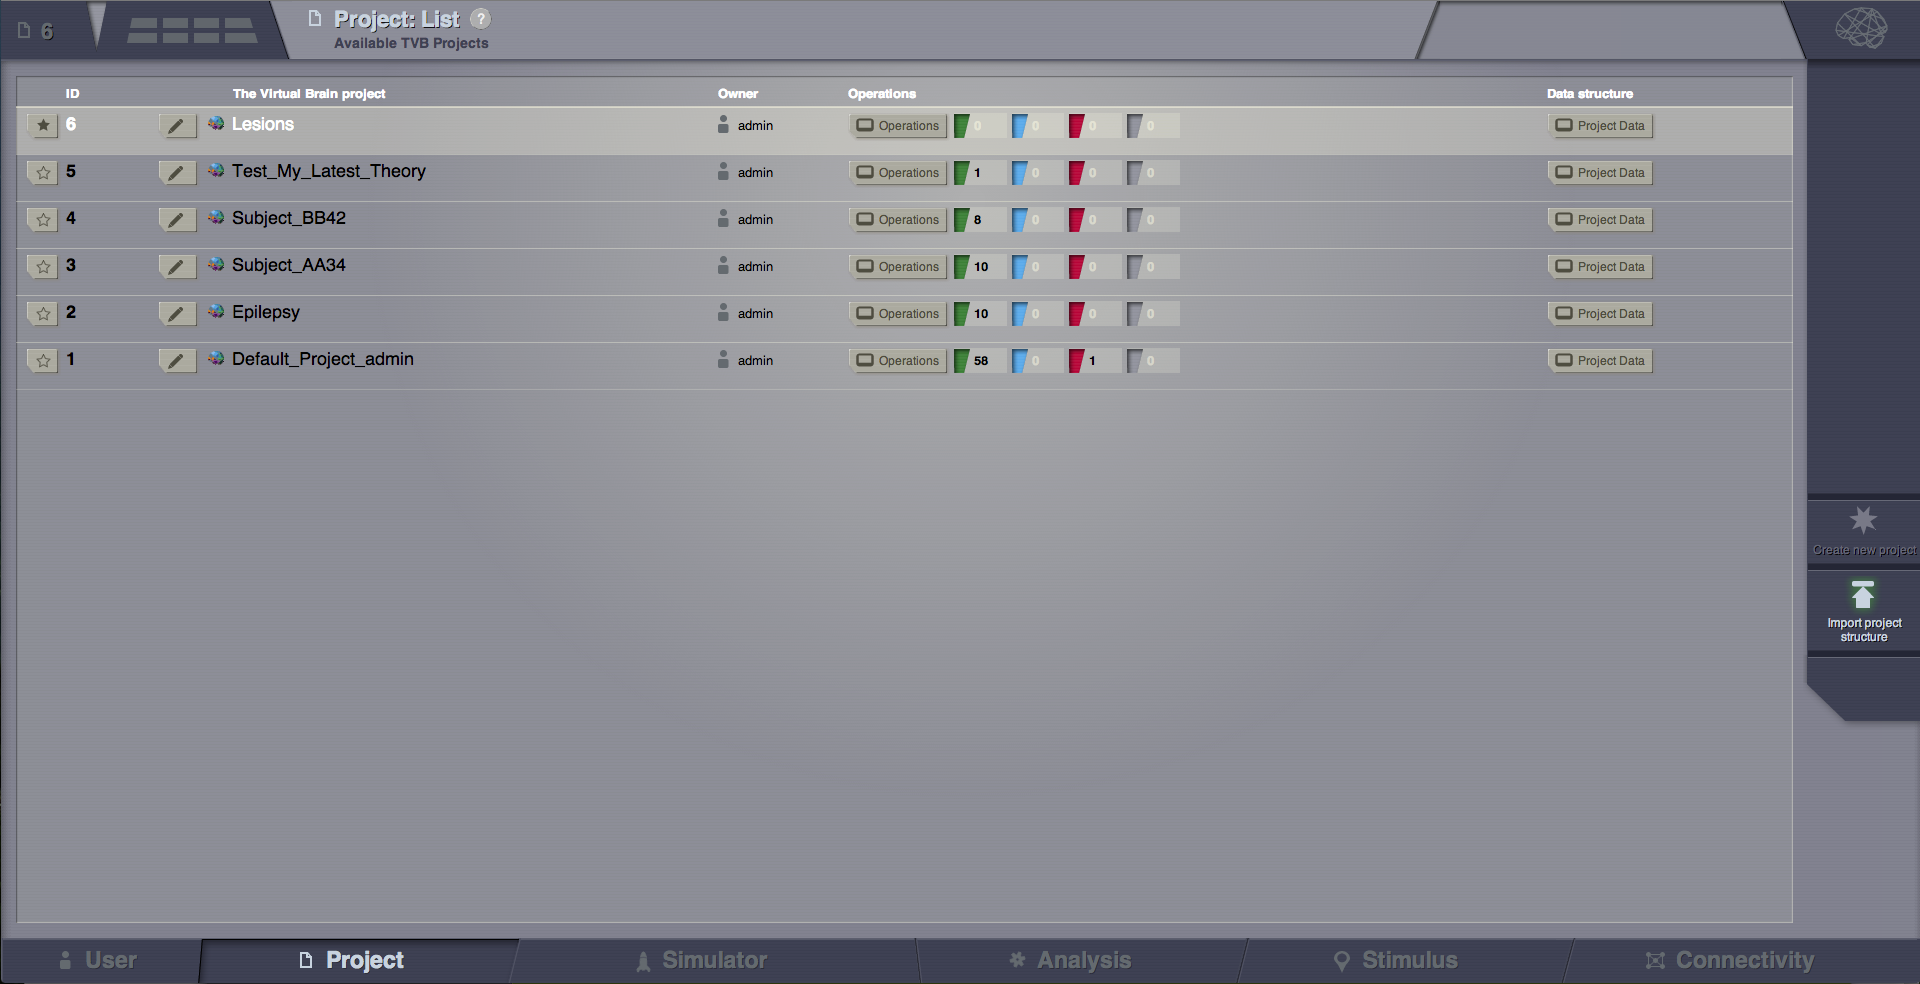
\includegraphics[width=0.50\textwidth]{images/ui_projects.png}}
	\qquad
	\subfloat[][]{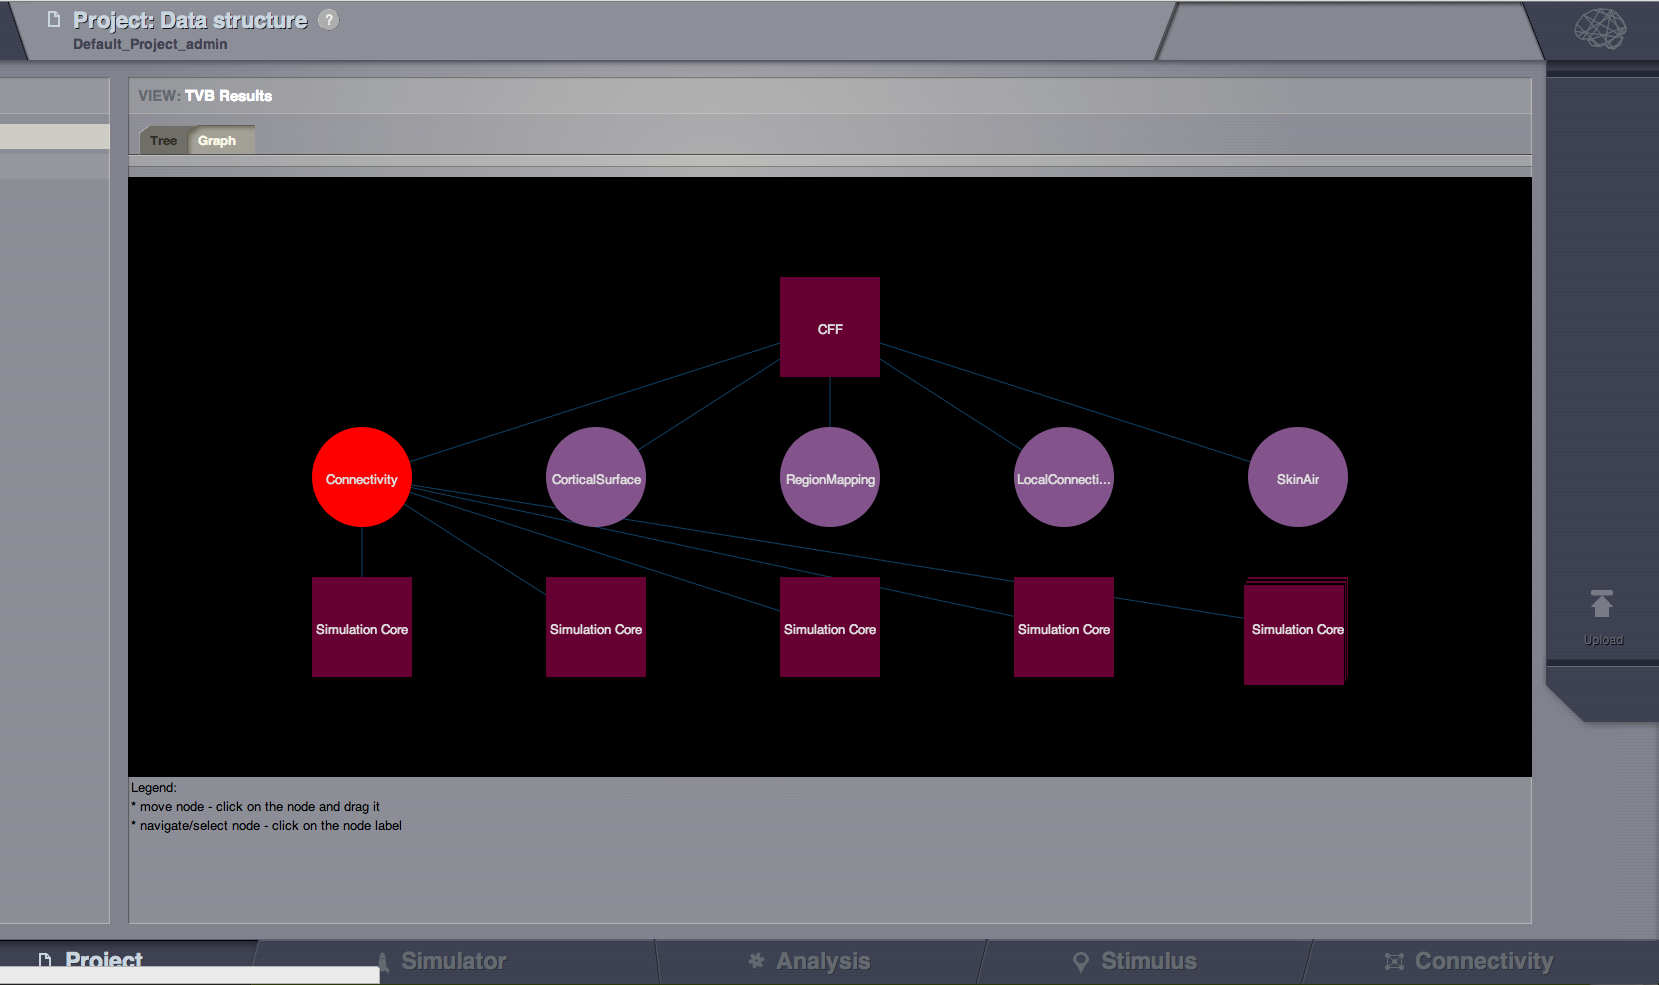
\includegraphics[width=0.434\textwidth]{images/ui_project_graph.png}}
	\\
	\subfloat[][]{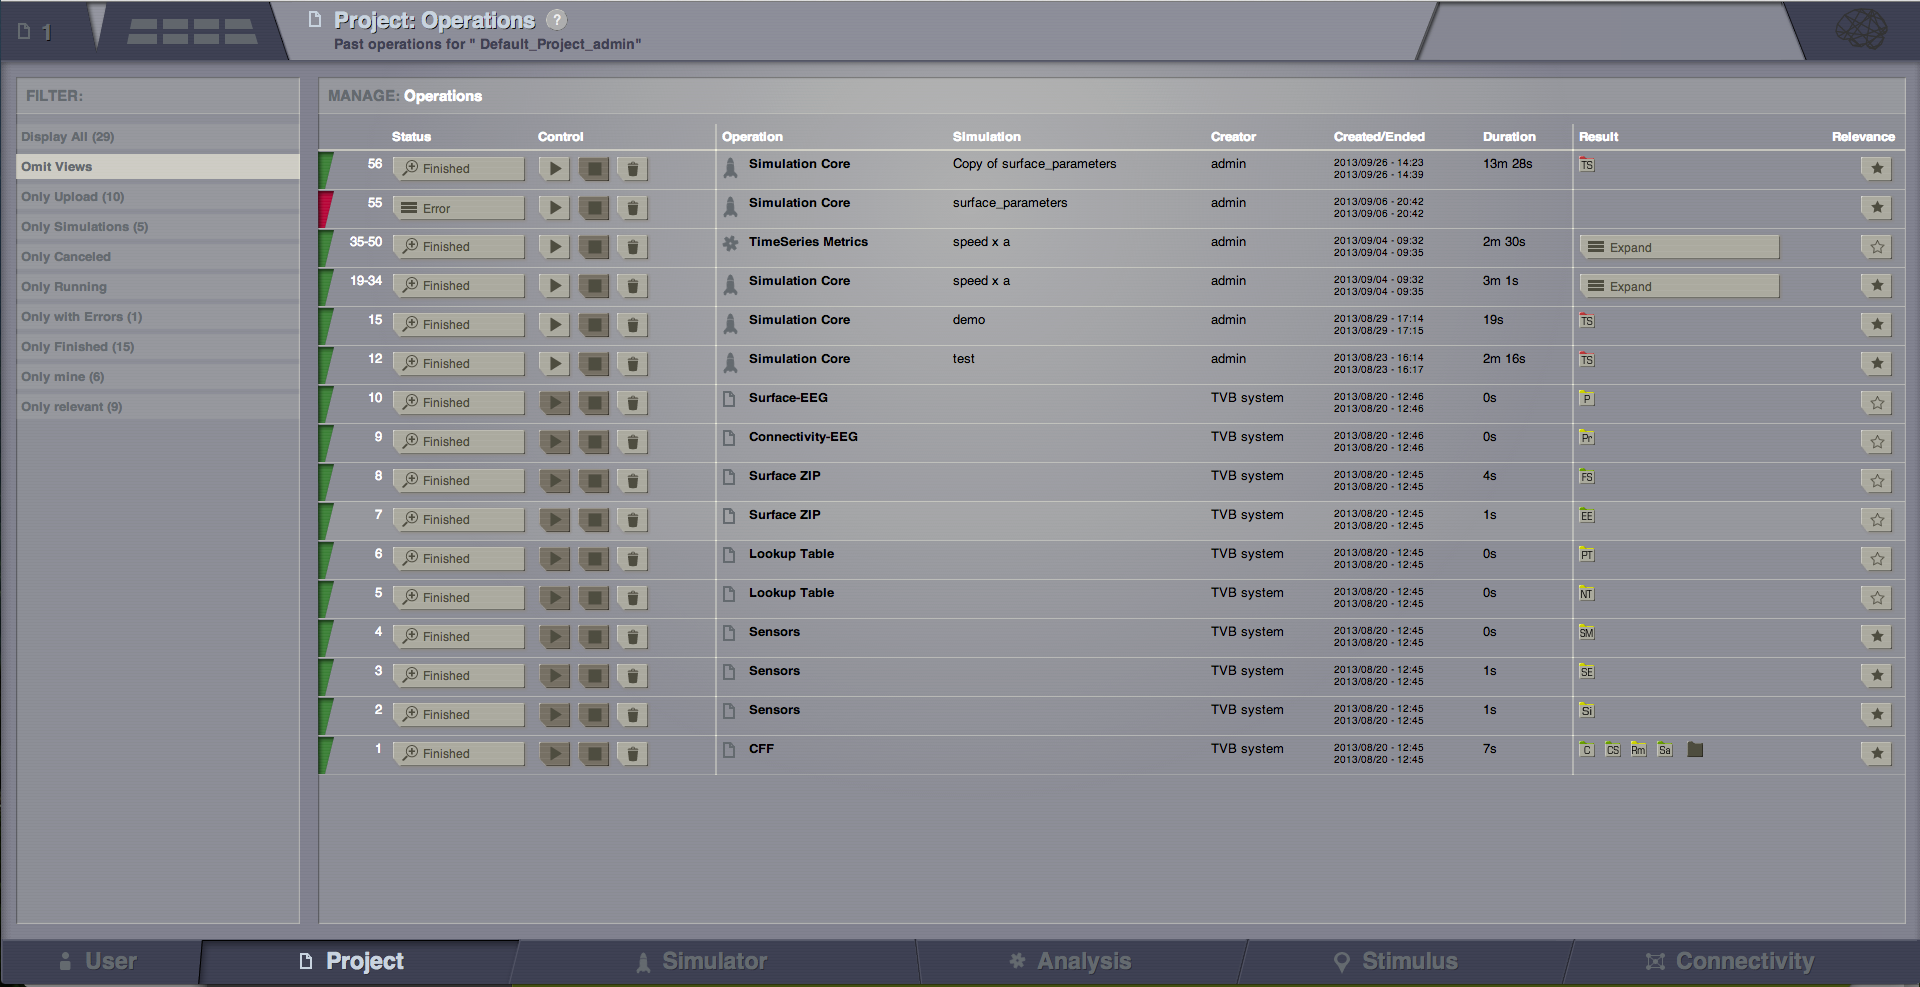
\includegraphics[width=0.50\textwidth]{images/ui_project_operations.png}}
	\qquad
	\subfloat[][]{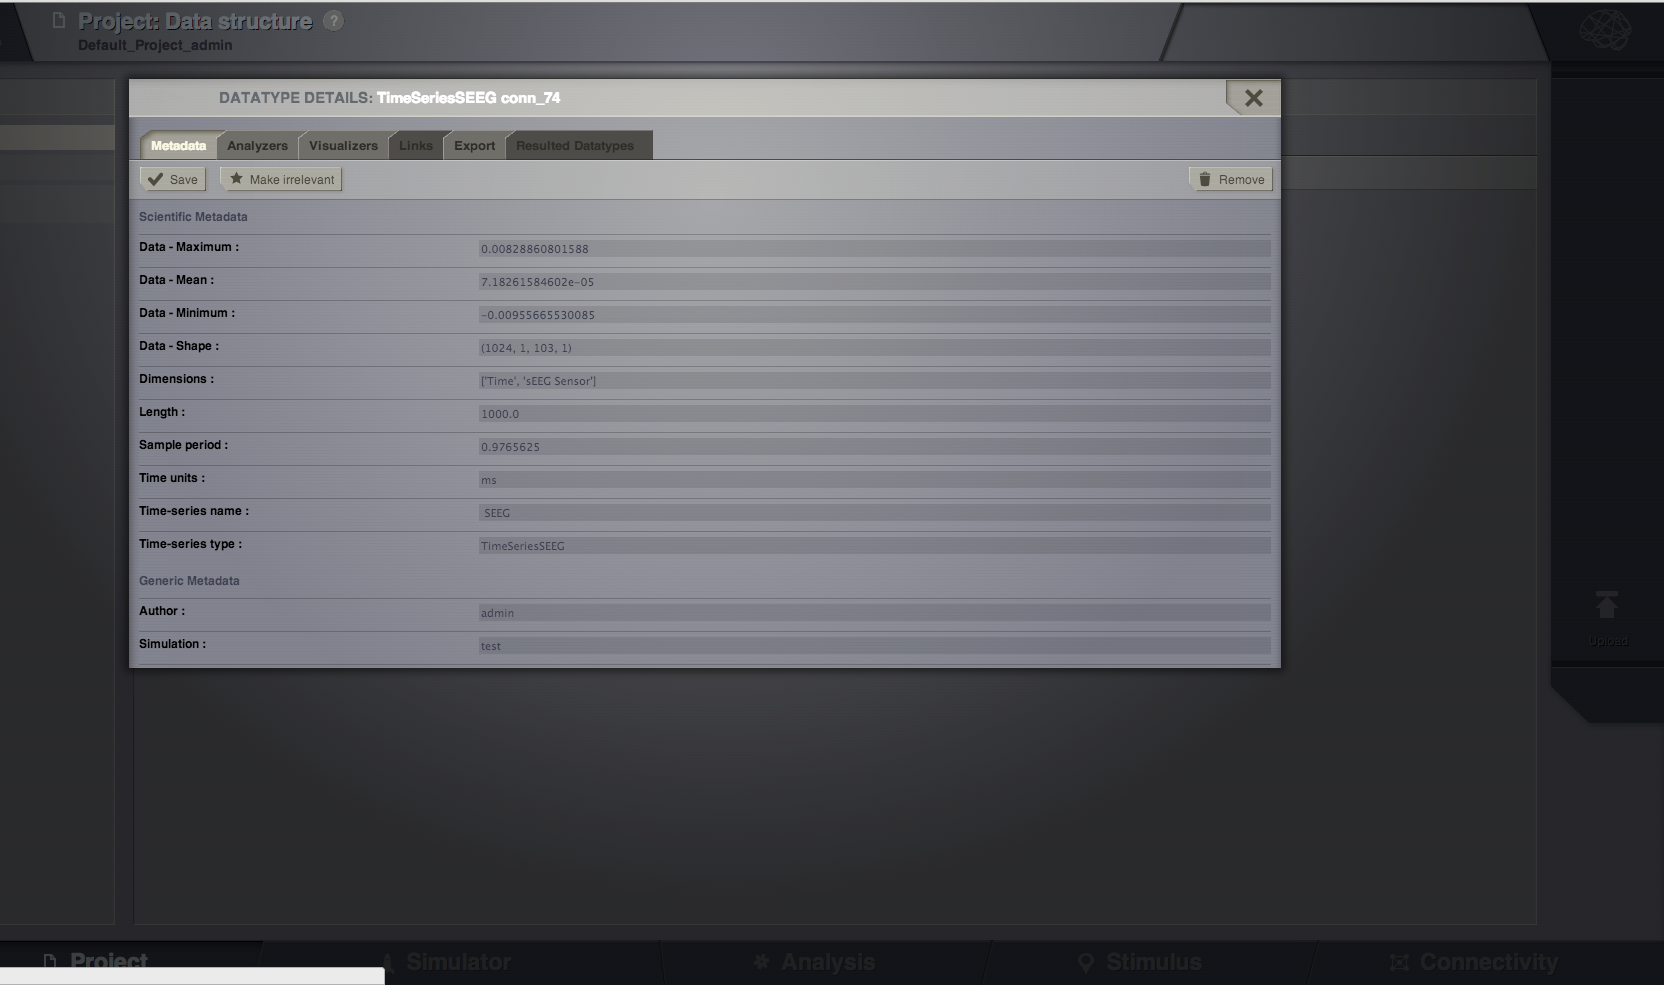
\includegraphics[width=0.434\textwidth]{images/ui_project_datatype_details.png}}
	\caption{\TVB Data Organization: 
	(A) View All Projects.
	(B) 2D graph display of operations with their input and output DataTypes .
	(C) View all Operations in current project with their status, duration, results, etc.
	(D) DataType details and further available operations for it. This menu becomes available after clicking a DataType result from several places in \TVB }
        \label{fig:project}
\end{figure*}

	\subsubsection{Simulator Interface}
	
	\subsubsection{Analysis \& Visualizers}

\TVB does not aim to compete at the analysis level with other tools in Neuroscience, 
highly specialized and with great history in data analysis, like  FSL or SPM. 
What we offer is a minimalist set or algorithms to post-process your 
simulated results (or even process imported patient measured scans) inside \TVB, mainly for quick validations.

We have created inside \TVB adapters for \emph{Fast ICA} from the python library \emph{sklearn}, 
we've implemented a python version of \emph{Fourier Spectral Analysis}, 
we have even wrapped the Matlab library \emph{BCT} \url{https://sites.google.com/site/bctnet/}, and others as analyzers.

For each of the DataTypes produced in \TVB, one or multiple visualizers are available.	
\TVB has couple of  visualizer types, each developed with the technology providing better support on the specific requirements for the visualization in course:

\begin{enumerate}

	\item \emph{WebGL viewers:} are based on \emph{HTML 5 Canvas} element and the \emph{gl} context. 
	These viewers offer 3D nice display, vectorial zoom support, user interaction with the scene (rotate, translate), quick response 
	(even when thousands of vertices and edges are to be manipulated) and good resolution for the images exported.
	
	\item \emph{SVG viewers:} offer great selection, zoom and scaling effects and extraordinary quality for the exported artifacts, while having 
	a relatively low number of elements to display on the page. 
	We use such viewers for manipulating and displaying TimeSeries, Covariance or Cross Coherence DataType results.
	
	\item \emph{MPLH5 viewers:} \emph{Matplotlib} has an \emph{HTML 5} backend that we use for viewing someof \TVB DataTypes (like Fourier or Wavelet)
	\url{https://code.google.com/p/mplh5canvas/}
	
	\item \emph{Other} simpler viewers are using JIT \url{http://philogb.github.io/jit/} or FLOT \url{http://www.flotcharts.org/} JS libraries.
	These are mainly 2D graph displayers for some simple \TVB generated data.

\end{enumerate}

 \begin{figure*}
	\subfloat[][]{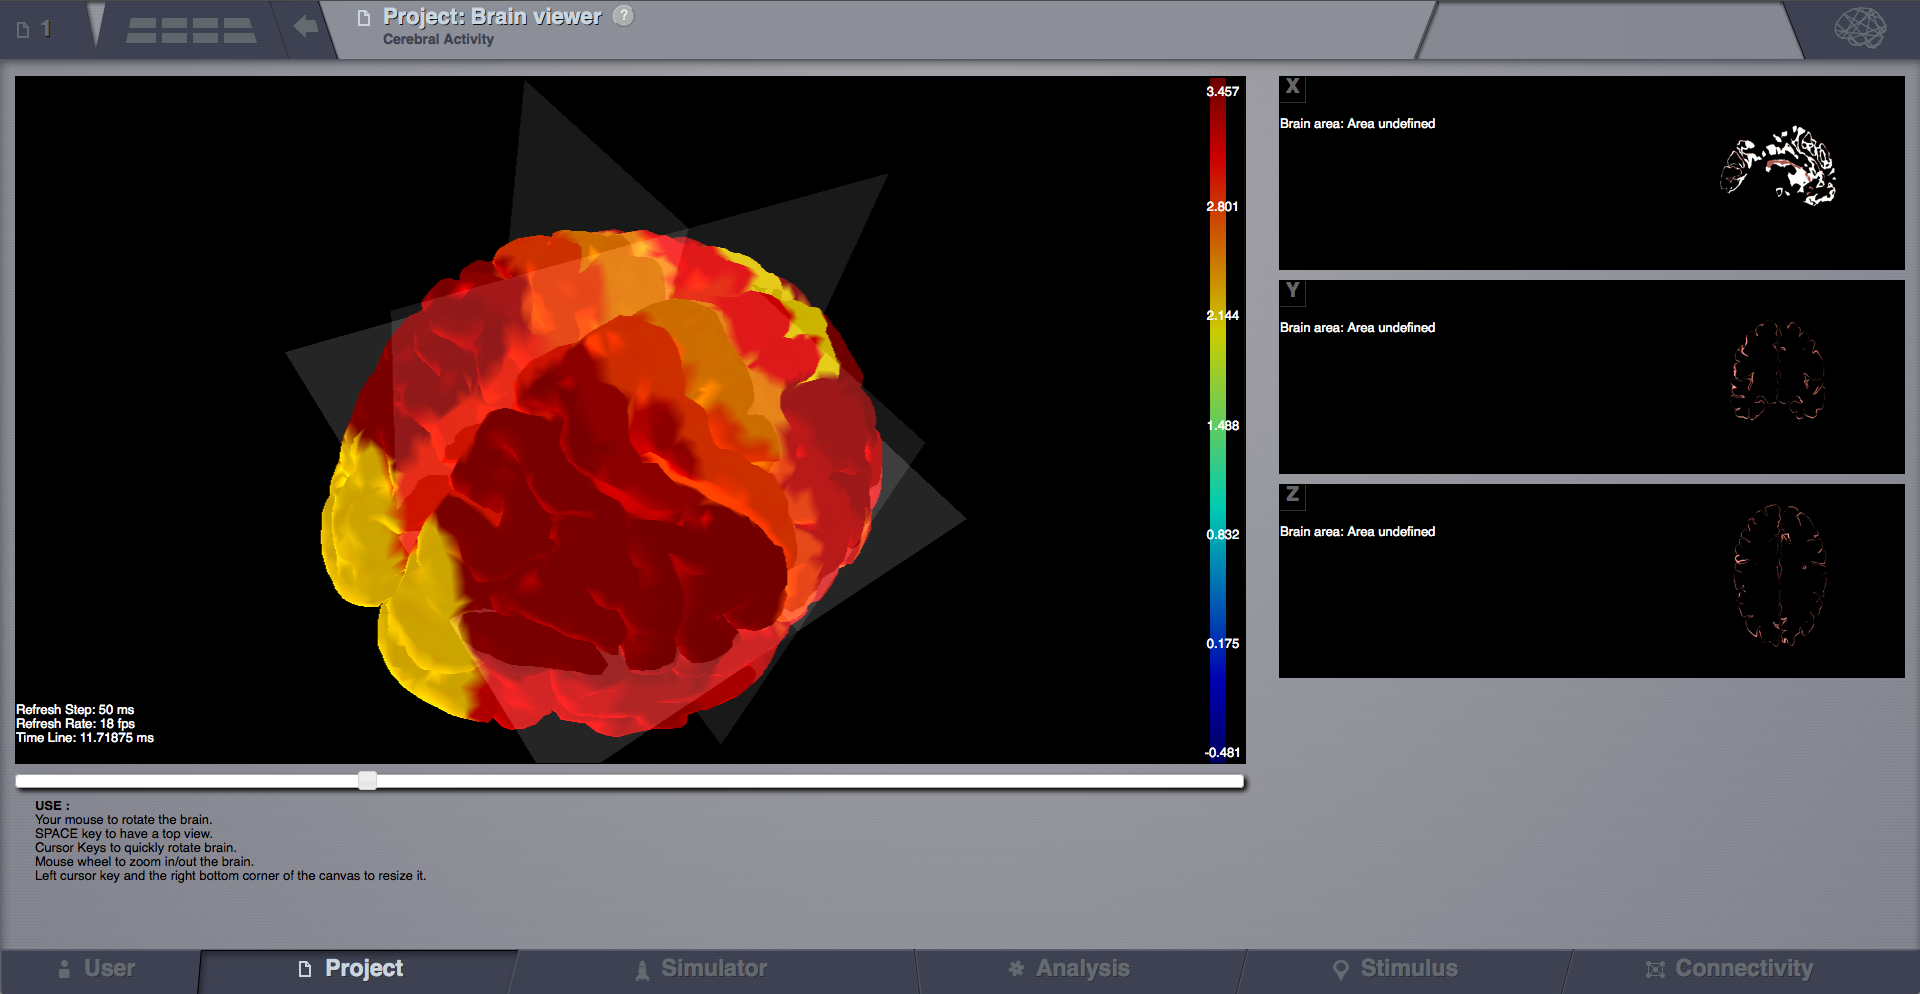
\includegraphics[width=0.48\textwidth]{images/ui_view_brain.png}}
	\qquad
	\subfloat[][]{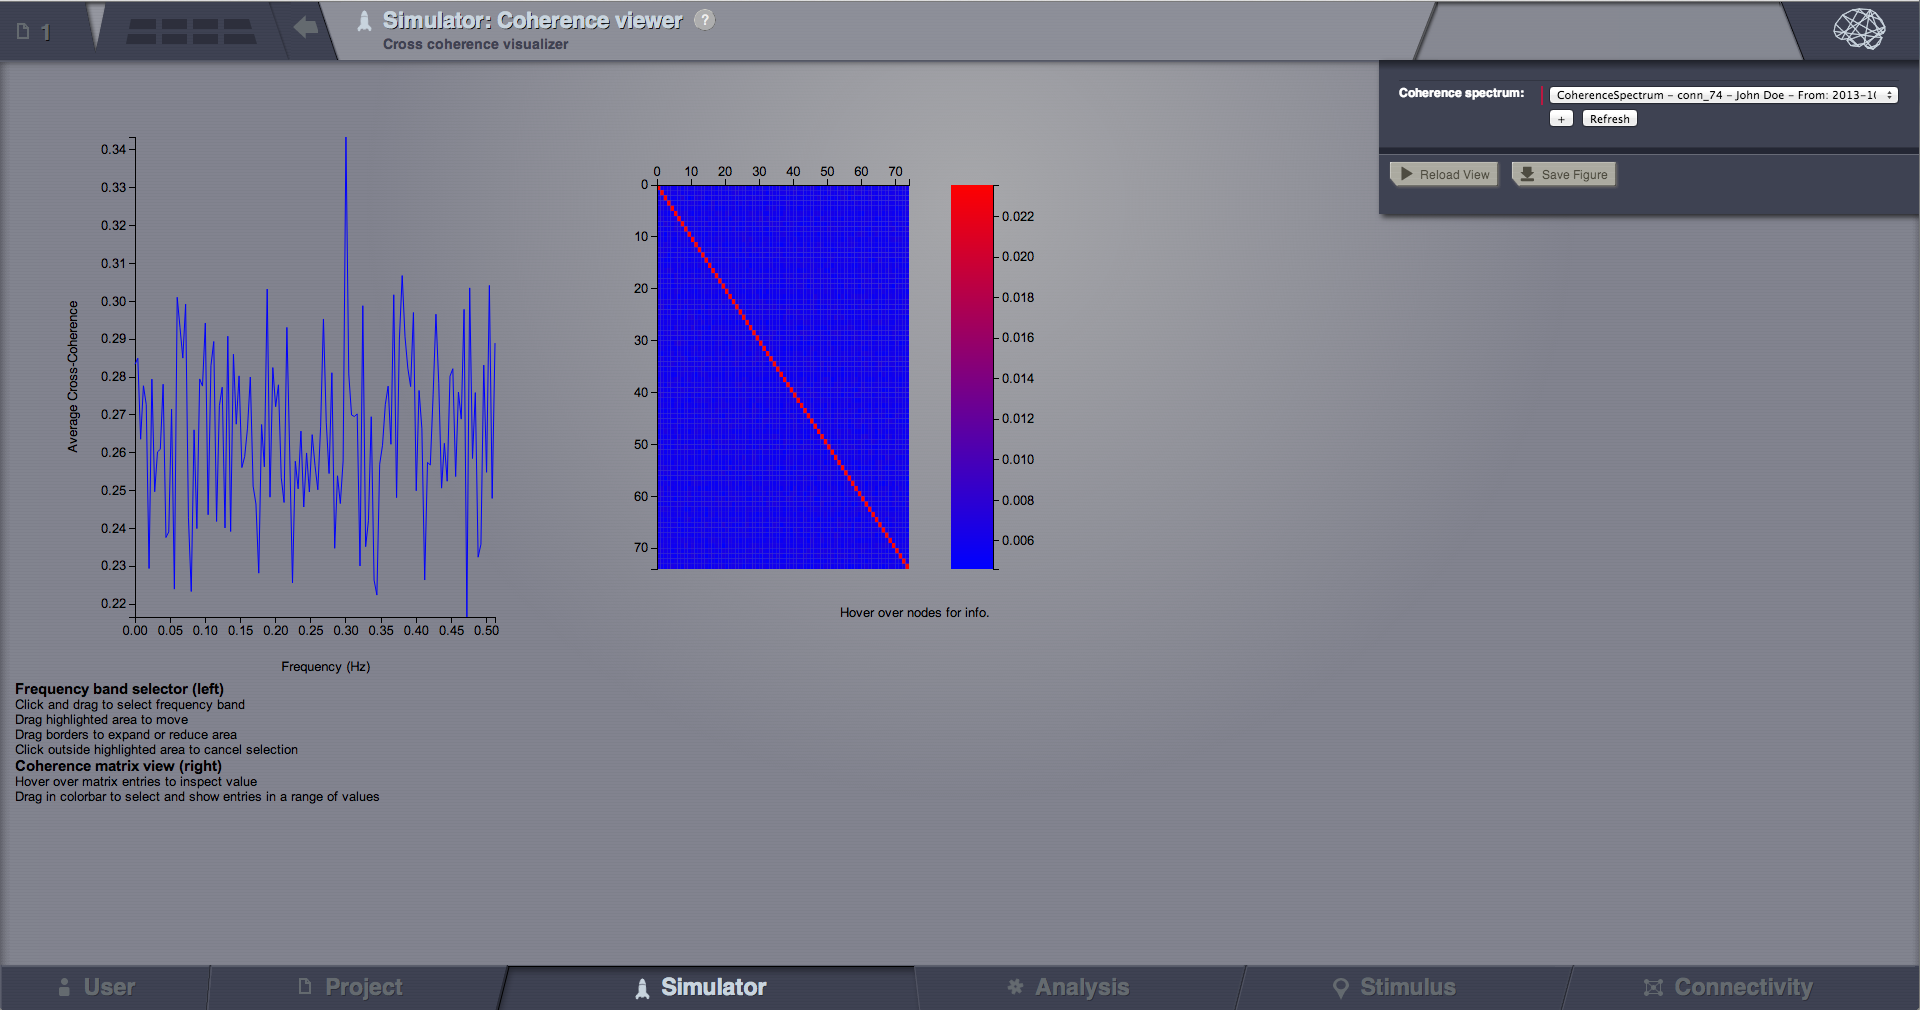
\includegraphics[width=0.48\textwidth]{images/ui_view_coherence.png}}
	\\
	\subfloat[][]{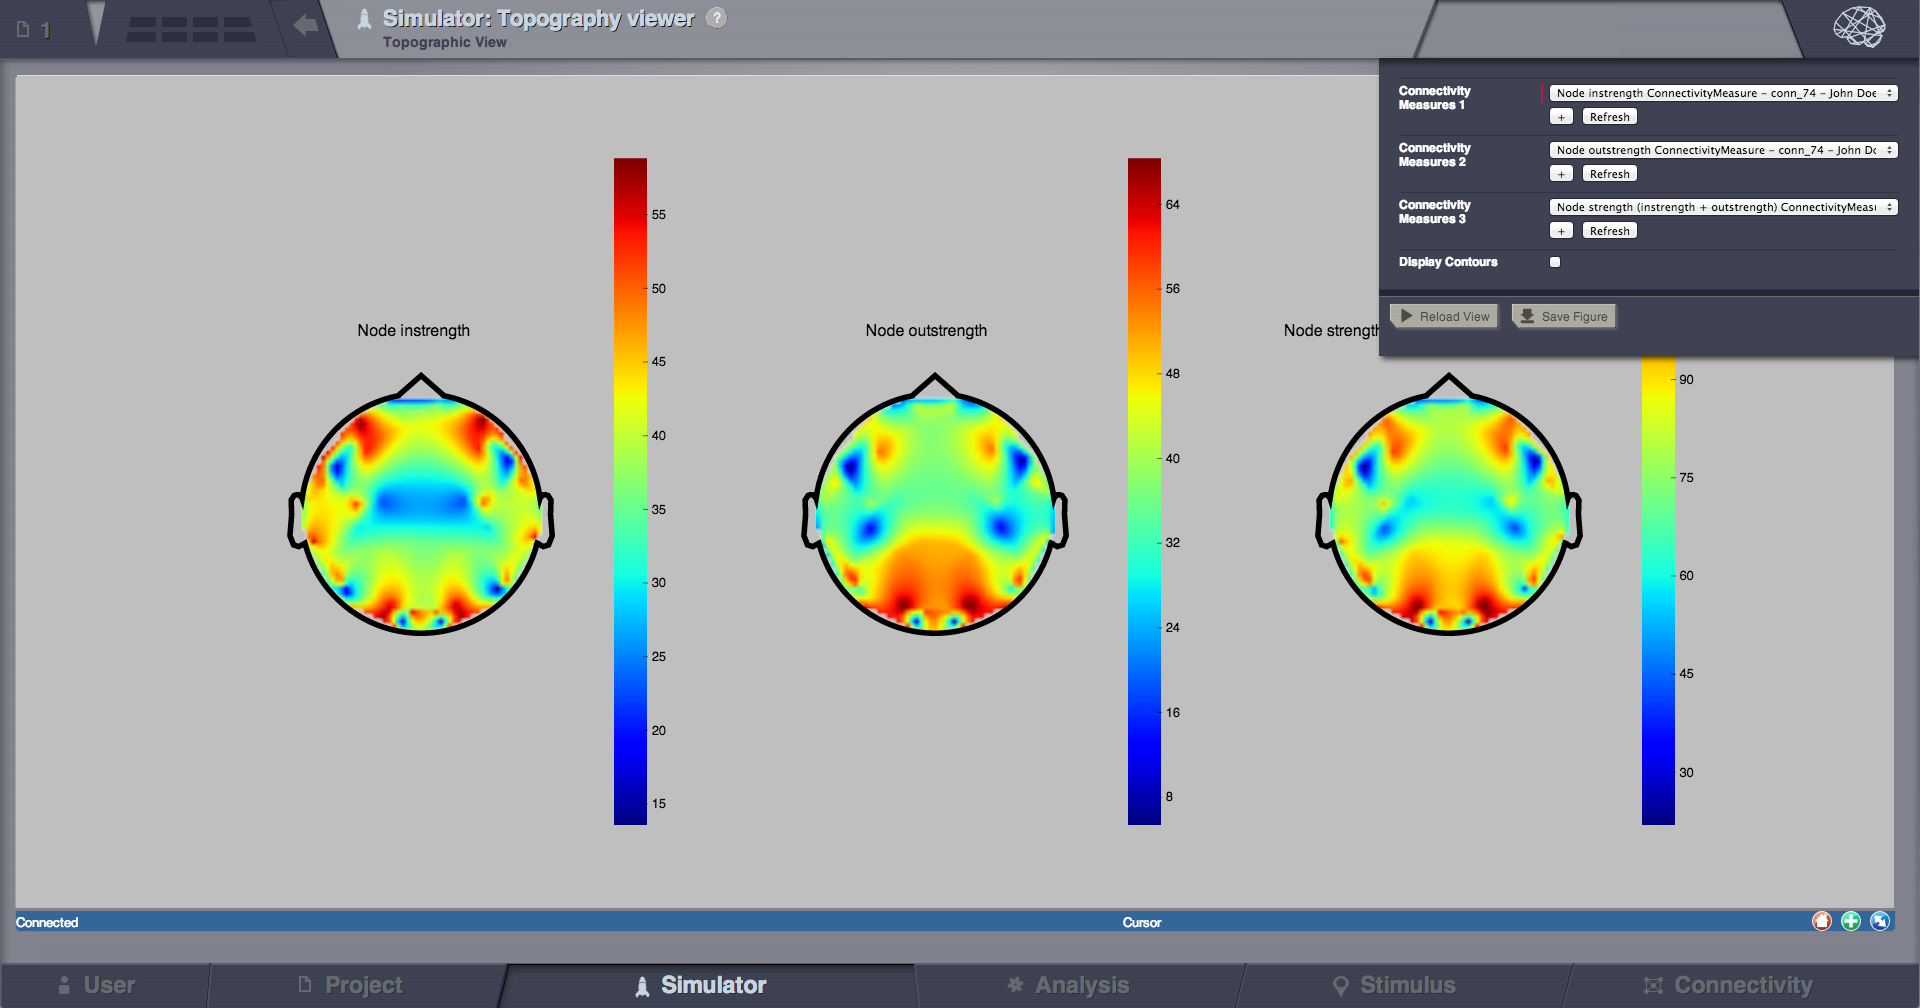
\includegraphics[width=0.48\textwidth]{images/ui_view_topo.png}}
	\qquad
	\subfloat[][]{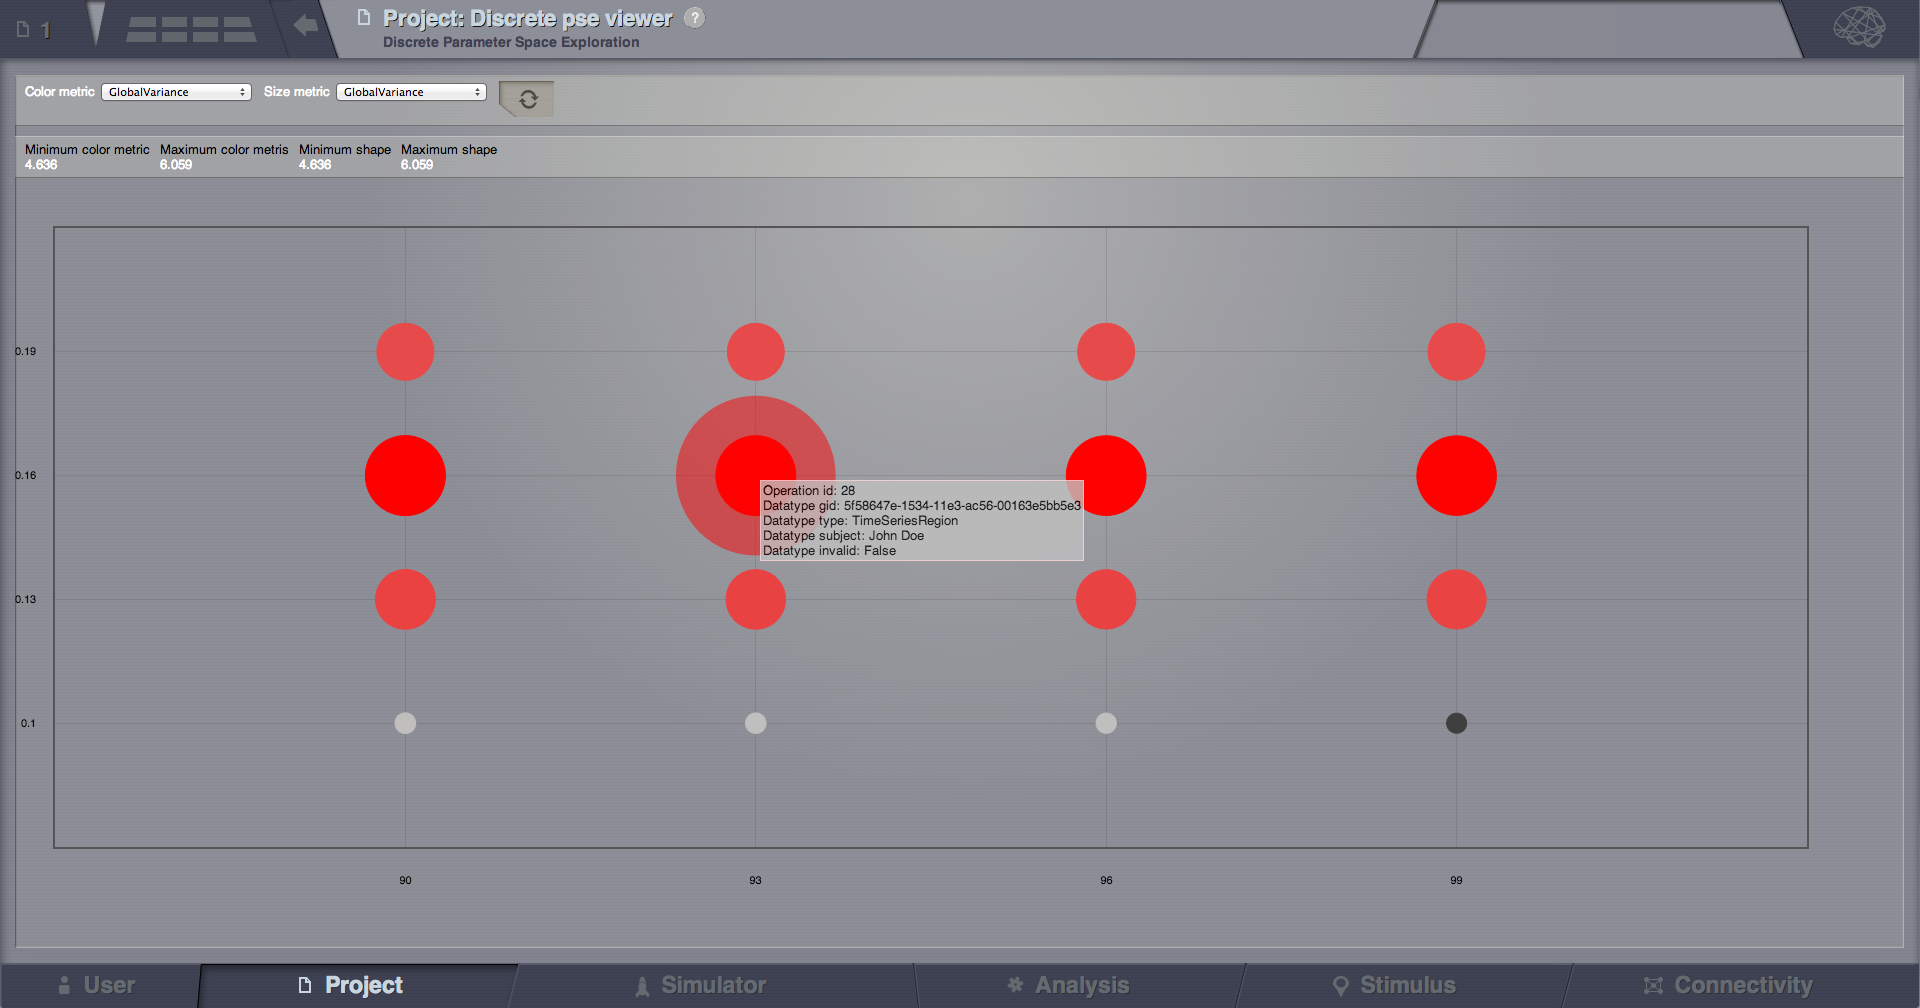
\includegraphics[width=0.48\textwidth]{images/ui_view_pse.png}}
	\caption{\TVB visualizers: 
	(A) WebGL: 3D display of region level simulated signal, mapped on a brain cortical surface
	(B) SVG: Cross Coherence
	(C) MPLH5:  Topograhic view with Connectivity in/out strength measures
	(D) FLOT: Parameter Space Exploration results grid}
        \label{fig:viewers}
\end{figure*}

	\subsubsection{Connectivity Tool}

Connectivity in the context of \TVB is a DataType, mapping structural information about a subject (real patient or theoretical model).
For editing and viewing a Connectivity, \TVB has a specific page, where the \emph{G-User} can manipulate connectivity strength and lengths 
starting from the granularity of an edge.

We do not store or use information about the exact anatomical path or a connection, only the region centers and connection weights and lengths.

 \begin{figure*}
 	\centering
	\subfloat[][]{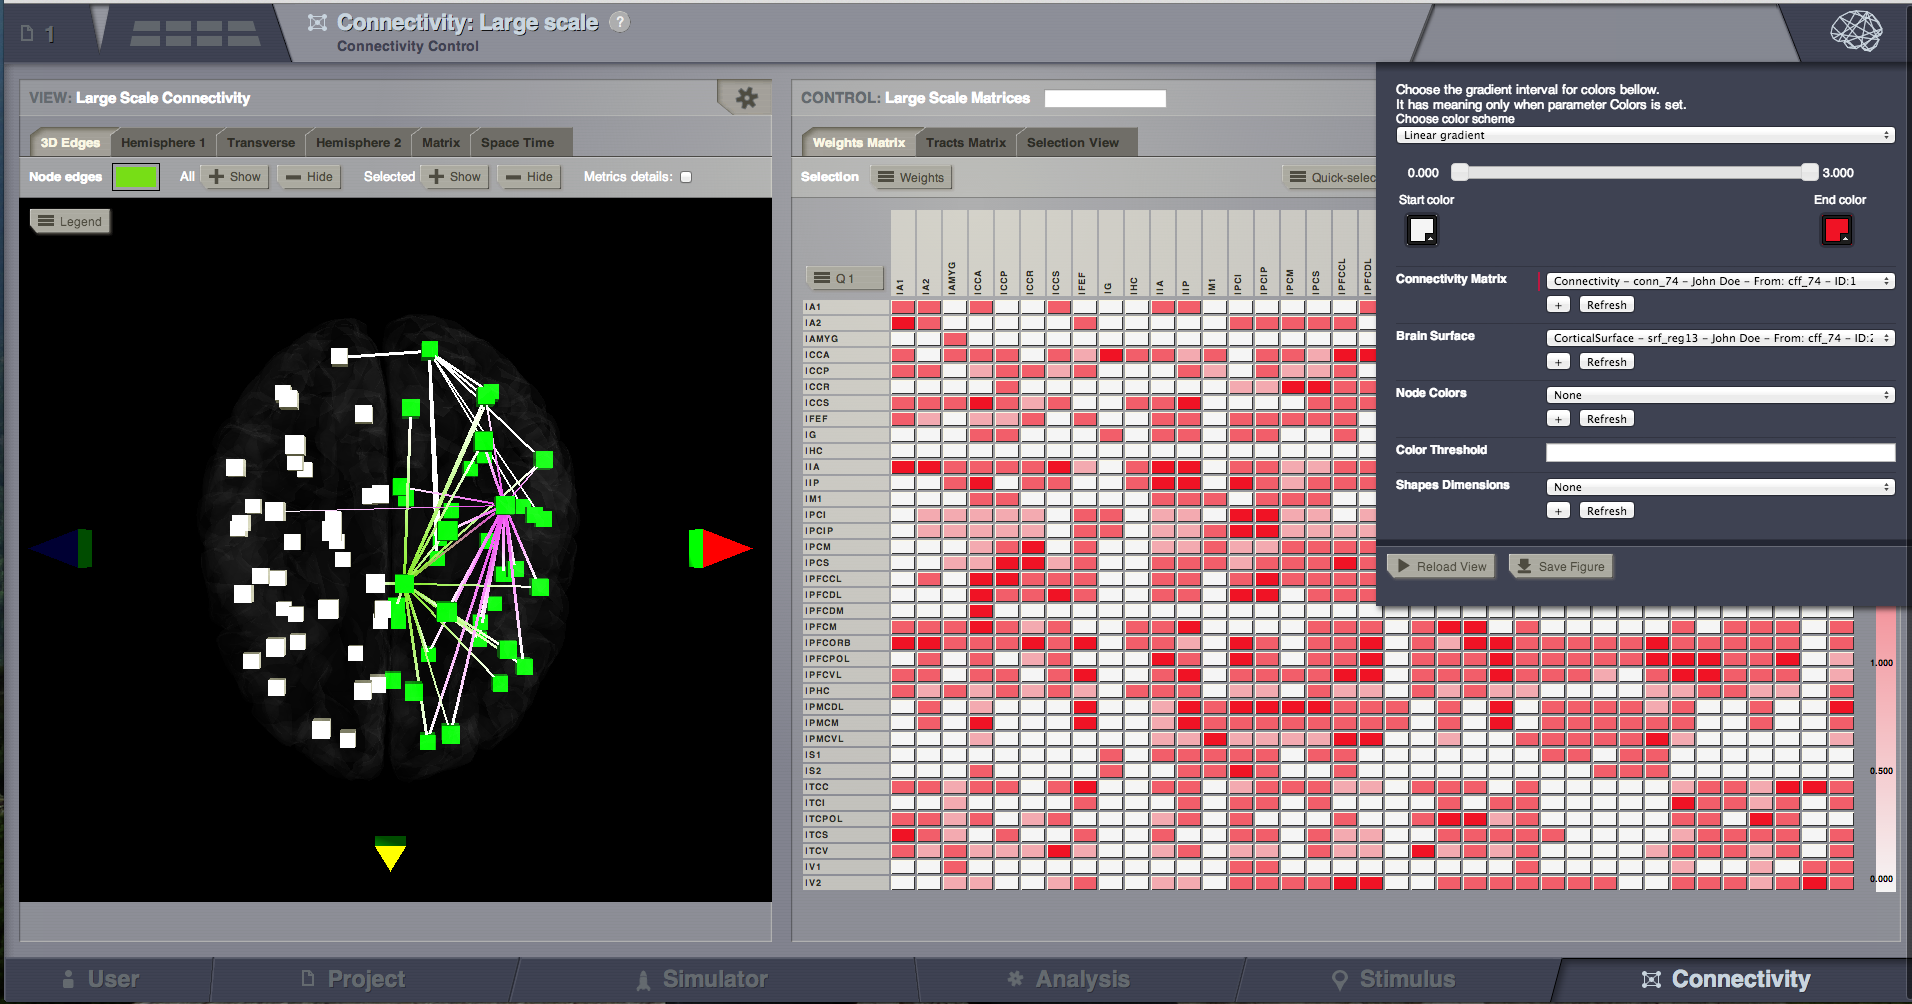
\includegraphics[width=0.48\textwidth]{images/ui_connectivity.png}}
	\qquad
	\subfloat[][]{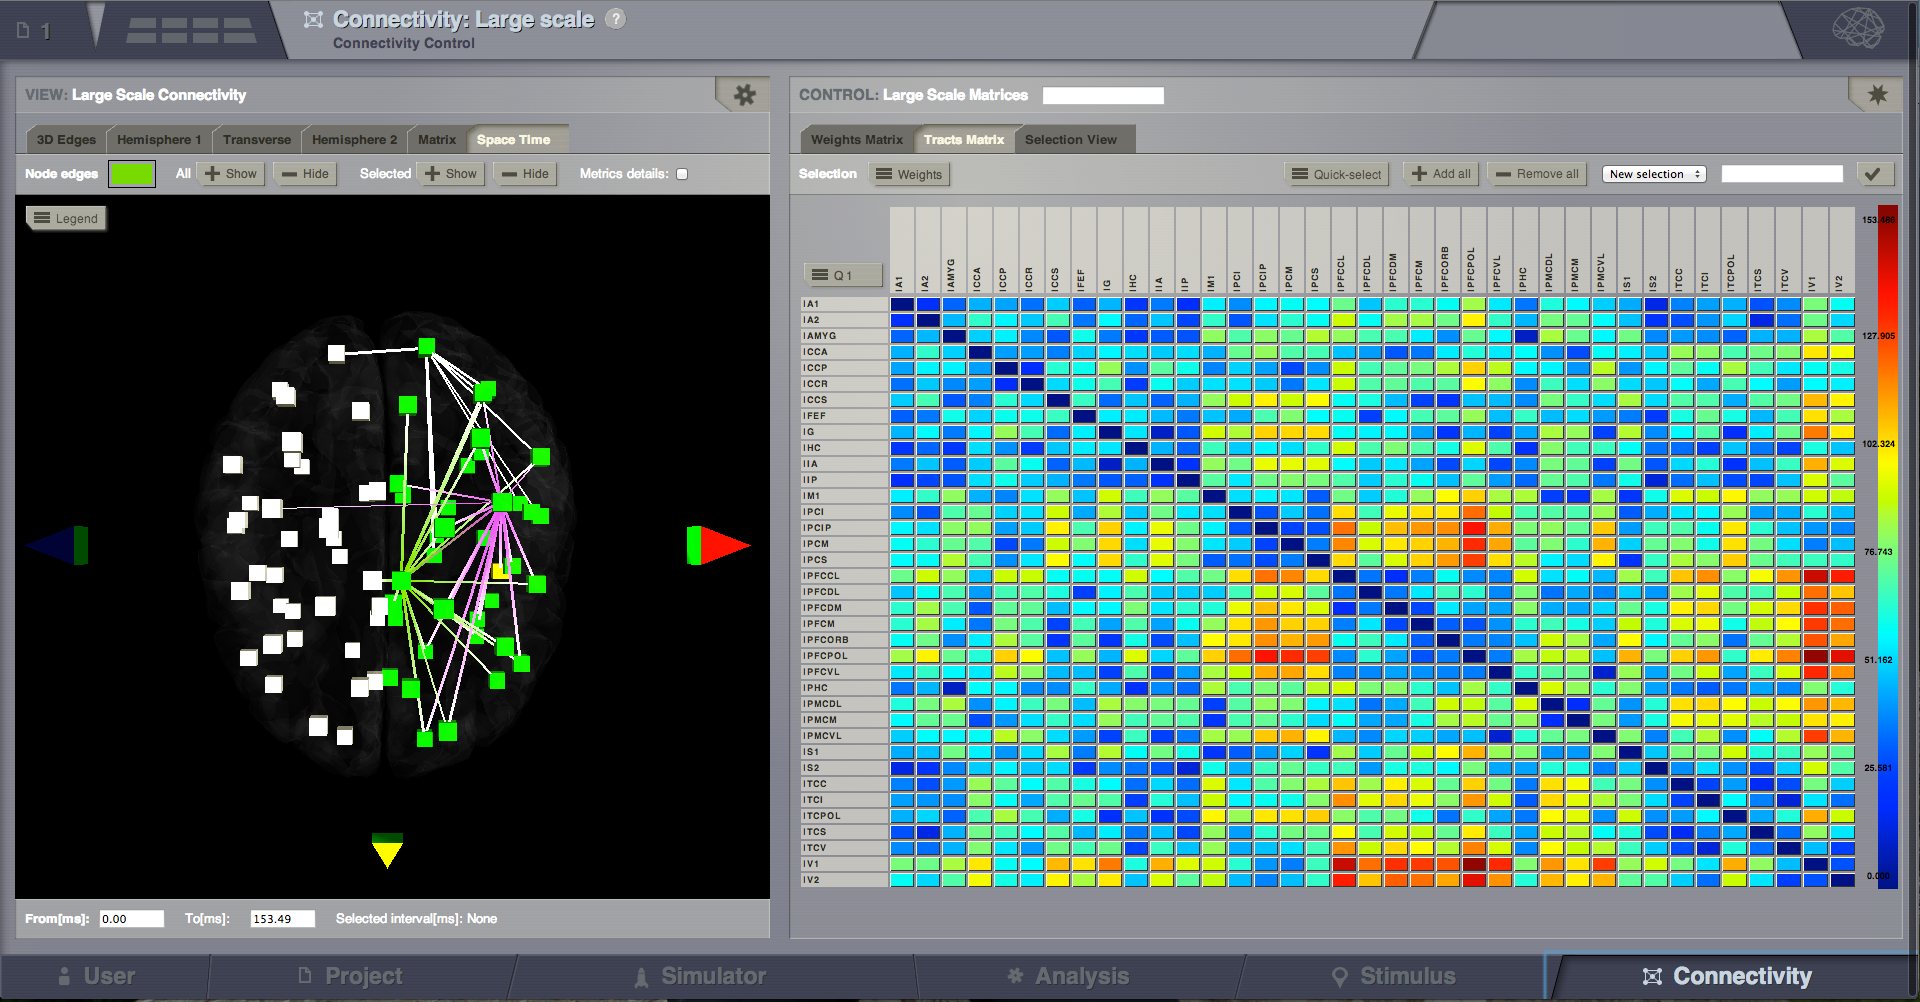
\includegraphics[width=0.48\textwidth]{images/ui_connectivity_delays.png}}
	\caption{Connectivity Tools: 
	(A) Left side: Displaying weighted connections between selection of nodes, with 3D manipulation.
	Right side: Editing weight connections, singular or bulk.
	(B) Left side: Show effect of connectivity delays when conductions speed is 1.
	Right side: Editing and displaying one quadrant from the matrix of connection tracts.}
        \label{fig:connectivity}
\end{figure*}



\subsection{Scripting Interaction}

\texttt{hello\_brain.py}
To give a basic feel for scripting \TVB simulations, we will 
walk through a simple example of a region-level simulation. We 
start with

\begin{lstlisting}
from tvb.simulator.lab import *
\end{lstlisting}

\noindent which is an all-in-one module making writing scripts
shorter, in the style of \texttt{pylab}, as it imports everything
from \texttt{pylab}, \texttt{numpy} and most of \TVB's simulator
modules. Next, we build a simulator object:

\begin{lstlisting}
sim = simulator.Simulator(
    model        = models.Generic2dOscillator(), 
    connectivity = connectivity.Connectivity(),
    coupling     = coupling.Linear(a=1e-2),
    integrator   = integrators.HeunDeterministic(),
    monitors     = (
        monitors.TemporalAverage(), 
    )
)
\end{lstlisting}

\noindent where we've employed a two dimensional oscillator
with default parameters, the default connectivity, a linear 
coupling function with a slope of $1e-2$, and deterministic
Heun integrator and a monitor that temporally averages the 
network dynamics before providing output.

While \TVB strives to keep modules independent of one another,
it is typical for mathematical dependencies to arise between, 
for example, the mass model and the integration time step, so
after configuring a simulator object, it is necessary to invoke

\begin{lstlisting}
sim.configure()
\end{lstlisting}

which results in walking the tree of objects, checking and 
configuring the constraints among parameters recursively.

The next step is to run through the simulation, collecting
output from the simulator. In this case, it is as simple as
\begin{lstlisting}
ys = array([y for ((t, y),) 
	      in  sim(simulation_length=3e2)])
\end{lstlisting}
\noindent where the simulator has been called, returning a 
generator which performs the integration and returns, for each
monitor, the current time and activity. In a case where EEG 
and fMRI monitors, for example, were used, we might write
\begin{lstlisting}
eeg, mri = [], []
for (t_eeg, y_eeg), (t_mri, y_mri) in sim(3e2):
    if y_eeg is not None:
	eeg.append(y_eeg)
    ...
\end{lstlisting}
\noindent Because fMRI and EEG monitors have very different
timescales, whenever one monitor return data and the others do
not, the others contain \texttt{None}, hence the check. Building
more complex logic in this loop would permit, for example, online
feedback and modification of connectivity. 

After the simulation loop has finished, you may wish to see the
result, following the previous listing, 
\begin{lstlisting}
plot(ys[:, 0, :, 0], 'k', alpha=0.1)
\end{lstlisting}
\noindent Here we note that \texttt{ys} is four dimensional. The 
simulator has the convention of treating  mass model state as a
three dimensional array of state variables by nodes by statistical
modes. Because \texttt{ys} is an array collected over time, the first
dimension is time, and the plot here is of each node's first state
variable, over time.

Many more demonstrations of the various features of the simulator
can been found in scripts distributed with the sources of \TVB, or 
browsed online at \url{https://github.com/the-virtual-brain/scientific_library/tree/trunk/tvb/simulator/demos}.
In the next section, we will go into detail about the different
components of the simulator.

